\RequirePackage[abort, l2tabu, orthodox]{nag}
\documentclass[pageno]{jpaper}

% standard LaTeX packages that do not interfere with hyperref
\usepackage{alltt}
\usepackage{amssymb}
\usepackage{booktabs}
\usepackage{caption}
\usepackage[draft]{fixme}
\usepackage{epstopdf}
\usepackage{flushend}
\usepackage{graphicx}
\usepackage[final]{listings}
\usepackage[sort&compress]{natbib}
\usepackage{tikz}
\usepackage[normalem]{ulem}
\usepackage{xspace}

% font selection
\usepackage{courier}
\usepackage{helvet}
\usepackage{mathptmx}
\usepackage{microtype}
\usepackage[mathscr]{euscript}

% hyperref itself
\usepackage{hyperref}

% standard packages that must be loaded after hyperref
\usepackage{bookmark}
\usepackage{verbatim}

% should be loaded after listings and subfig
\usepackage{cleveref}
\usepackage{multirow}
\usepackage{xfrac}

% custom packages for this paper
\usepackage{xcolor}

%\DeclareCaptionType{copyrightbox}

\renewcommand{\cite}[1]{%
  \PackageError{natbib}{%
    The \string\cite\space{} command is ambiguous; use
    \string\citet\space{} or \string\citep\space{} instead}{}}

\renewcommand{\autoref}[1]{%
  \PackageError{cleveref}{%
    Do not use \string\autoref.  Use \string\cref instead, or use
    \string\crefrange for ranges of referenced items}}

\renewcommand{\hline}[1]{%
  \PackageError{booktabs}{%
    Do not use \string\hline.  Use \string\toprule, \string\midrule,
    or \string\bottomrule\space instead depending on where in the
    table the line appears}}

\newcommand{\email}[1]{\href{mailto:#1@cs.cmu.edu}{#1}}

% cleveref configuration
\crefname{figure}{Figure}{Figures}
\crefname{section}{Section}{Sections}
\crefname{table}{Table}{Tables}

\hyphenation{test-case}

% lst configuration
\lstdefinelanguage{example}{%
  morekeywords={xyz},
}

\lstset{
  basicstyle=\sffamily,
  columns=fullflexible,
  numbersep=5pt,
  numberstyle=\scriptsize,
  showstringspaces=false,
  language=example,
  escapeinside={/*@}{@*/},
  belowcaptionskip=1\baselineskip,
  language=C,
  showstringspaces=false,
  keywordstyle=\bfseries,
  commentstyle=\itshape,
}


\urlstyle{sf}

\pdfpagewidth=8.5in
\pdfpageheight=11in


% Custom commands
\newcommand{\Tool}{\textsc{XYZ}\xspace}

%\sloppy
% start doc
\begin{document}

\title{
  \textsc{\LARGE Midway Report\\
  \Large Automatic Tuning of DBMS using Machine Learning\\
  \large CMU 10-701: Machine Learning (Fall 2014)}
}

\author{Joy Arulraj \hspace{0.1 in} Ram Raghunathan \hspace{0.1 in} \\
{\{\email{jarulraj}, \email{rraghuna}\}}}

\date{}
\maketitle


\begin{abstract}
Modern database systems are highly configurable and must support a
wide variety of workloads. However, \textit{tuning} these systems is
challenging. Configuration assistants like Microsoft's AutoAdmin
\citep{agrawal03} allow administrators to use statistics and
suggestions from the database
system to guide the physical design of the database. However, these methods
still require experienced administrators and prior knowledge about the
workload. We seek to apply machine learning methods to automate database
system tuning with minimal user input and knowledge by matching
workloads to representative benchmarks. In this midway
report, we discuss the our progress on the workload mapping problem.
\end{abstract}

\section{Introduction} \label{sec:intro}

\subsection{Motivation}

DBMS tuning is a niche skill that involves configuring the DBMS suitably for the
underlying hardware as well as guiding the physical design of the database.
Doing these tasks effectively requires a deep knowledge of the SQL workload to
be run on the DBMS, extensive prior experience in DBMS tuning, as well as
significant amounts of time-consuming experimentation with candidate
configurations. This issue is prevalent across several widely used database
management systems. For instance, Robert Hass, a core developer of PostgreSQL, 
stated that \citep{hass12} :

\begin{displayquote}
``On one test, involving 32 concurrent clients, I found that wal\_buffers = 64
MB doubled performance as compared with wal\_buffers = 16 MB; however, on
another system, I found that no setting I tried produced more than a 10 \%
improvement over the auto-tuning formula.'' 
\end{displayquote}

We therefore propose applying machine learning methods to automate the process
of tuning the DBMS for a particular workload on a specific machine.

\subsection{Problem definition}

We address two problems in this project.
First, we try to \textit{map} a given workload comprised of
a set of SQL transactions to a standard database benchmark workload. 
This problem is independent of the underlying DBMS or hardware configuration.
This will allow us to use prior knowledge about the standard 
benchmark gained from previous DBMS deployments. 

We collect features that characterize the SQL workload as well as 
DBMS statistics.
We then use unsupervised techniques like clustering
and supervised techniques like decision-trees 
for mapping the workload.
Performance analysis of the resulting classifier is done via
cross-validation.

Second, we plan to \textit{estimate} the DBMS performance given a 
DBMS configuration, hardware setup and SQL workload. 
This is done with supervised techniques like 
Gaussian process regression.
We use the lasso regression estimator to identify key features 
that influence the throughput and average transactional latency 
of the DBMS.
Performance analysis of the estimator is also done using 
cross-validation.
We describe our progress on solving these problems in this report.

The goals of this project are the following : 
\begin{itemize}
  	\item to create a workload mapper that maps an arbitrary SQL workload to a
well-known standard benchmark
	\item to estimate the performance metrics of a DBMS given a workload and
configuration pair
\end{itemize}

We first describe how we generate the dataset in \cref{sec:data_set}. 
Then, we focus on the feature extraction problem in \cref{sec:features}.
We describe our experimental setup and dataset information in
\cref{sec:eval}. The evaluation results obtained for the classification
problem and the estimation problem are shown in \cref{sec:classfication}
and \cref{sec:estimation} respectively. Finally, we present the 
conclusions of this project in \cref{sec:conclusion}.
%\input{section/motivation}
%\input{section/data_set}
\section{Data Set} \label{sec:data_set}

The dataset required for this project would ideally comprise of a 
collection of real world SQL workloads, DBMS configurations and performance
metrics. Collecting and curating such a dataset is itself an interesting
problem.
However, in this project, we first want to experiment with a smaller dataset
to better understand the features relevant for our learning problem.
Therefore, we chose to generate the dataset using
OLTP-Bench~\citep{oltpbench14}, an extensible DBMS benchmarking framework.
We use the SQL workloads of standard benchmarks already available
in OLTPBench. 

We generate more synthetic variants of these workloads for training and
testing purposes. As we mentioned earlier, while this synthetic data will not be
representative of real-world workloads, we feel it is a good starting point for
evaluating viability of the approach outlined above.
We extract several features from the workload such as types of database queries,
distribution of query types, and table access patterns using 
a workload analyzer. We hook this analyzer into Postgres~\citep{postgres91} to collect 
features from the DBMS.

The key reasons for why we use OLTP-Bench framework to generate the dataset 
are the following:

\begin{itemize}
  \item It supports several relational DBMSs through the JDBC interface
  including Postgres, MySQL, and Oracle.
  \item It allows us to control the workload mixture in a benchmark. For
  instance, we can adjust the percent of read and update transactions in 
  the YCSB~\citep{ycsb} benchmark to generate different variants of the workload.
  \item It supports user-defined configuration of the rate at which the
  transaction requests are submitted to the DBMS. This allows us to emulate
  different world workloads with varying degrees of concurrency.
  \item It exposes statistics that are complementary to the 
  internal statistics of the DBMS~\citep{postgres14}. We extract features from
  these statistics.
\end{itemize}

We implemented a dataset generator that runs different benchmarks supported
by OLTP-Bench on a Postgres DBMS. After every workload execution, we
collect statistics from the DBMS as well as from the testbed. We alter the
workload mixture in all the benchmarks to generate different variants and
emulate real world workloads. The key characteristics of the benchmarks
that we use for generating the dataset are presented in \cref{tab:benchmarks}.

\begin{table*}[ht!]
  \centering
  \begin{adjustbox}{max width=\textwidth}
  \begin{tabular}{l|lllllllll} \toprule
   Benchmarks & Tables & Columns & Pr. & Indexes &	Fr. & 
   Txn. & \# of & Application  & Attributes  \\
   & & & Keys & & Keys & Types & Joins  & domain & \\
   \midrule
	AuctionMark 	& 16 	& 125  &	16 &	14 &	41 &	10 &	10 &	Online &
	Non-deterministic\\
	& & & & & & & & Auctions &  heavy transactions \\
	Epinions 		& 5 	& 21   & 	2  &	10 &	 0 & 	9  &	3  &	Social  & Joins over
	many-to- \\
	& & & & & & & & Networking & many relationships  \\
	%JPAB 	7 	68 	6 	5 	3 	4 	N/A 	Object-Relational Mapping 	Bursts of random%reads, pointer chasing 
	%ResourceStresser 	4 	23 	4 	0 	0 	6 	2 	Isolated Resource Stresser 	CPU-,disk-, lock-heavy transactions 
	SEATS &	10 &	189 &	9 	& 5 	& 12 	& 6 &	6 &	Online Airline  &
	Secondary indices queries\\
	& & & & & & & & Ticketing & foreign-key joins \\
	TATP &	4 	& 51 &	4 &	5 &	3 &	7 &	1 &	Caller Location  &	Short, read-mostly\\
	& & & & & & & & App & non-conflicting\\
	& & & & & & & & &  transactions\\
	TPC-C &	9 &	92 &	8 &	3 &	24 &	5 &	2 &	Order Processing & Write-heavy
	transactions\\
	Twitter &	5 &	18 &	5 &	4 &	0 &	5 &	0 &	Social Networking & Client-side joins \\
	& & & & & & & & & on	graph data \\
	Wikipedia &	12 &	122 &	12 &	40 &	0 &	5 &	2 &	Online &	Complex	transactions \\ 
	& & & & & & & & Encyclopedia & large data, skew  \\
	YCSB &	1 &	11 &	1 &	0 &	0 &	6 &	0 &	NoSQL store &	Key-value queries \\
   \bottomrule
   \end{tabular}
   \end{adjustbox} 
\caption{Key characteristics of the benchmarks used in our evaluation. ``Pr. key''
denotes primary key and ``Fr. key'' denotes foreign key.}
\label{tab:benchmarks}
\end{table*}



\section{Feature Extraction} \label{sec:features}

We collect 3 types of features from both the DBMS as well as the benchmarking
framework.

\subsection{Features from OLTP-Bench }

  After executing the benchmark, we obtain statistics about the latency and
  throughput delivered by the DBMS.
  This includes both temporal performance metrics as well as aggregate metrics. 
  We then record the size of the workload also known as the
  \textit{scalefactor}.
  The \textit{isolation level} of the DBMS correlates strongly with performance
  metrics Stricter isolation levels like ``serializable level'' correlate with lower
  performance because the DBMS needs to maintain the constraints regarding
  the visibility of effects of concurrent transactions. 
  
  We also record the type
  of DBMS used. Although currently we focus only on Postgres, 
  we anticipate this tool to be useful for other DBMSs as well.   
  We also record the expected label i.e. the benchmark name. This is used for
  evaluating the accuracy of our classification algorithms.  
  
\subsection{Static parameters from Postgres}

  Static parameters are features that do not vary over every execution. This
  primarily includes the configuration parameters of the DBMS and the hardware
  setup.
  For example, these are some of the static parameters that we use as features:\\
   
  \begin{itemize}
    \item {Size of shared memory buffers: This impacts the performance of
    memory-intensive queries significantly.}
    \item {Background writer delay: The background writer issues writes of
    dirty shared buffers to disk. This increases the net overall I/O load but
    allows server processes to avoid waiting for writes to finish.}
    \item {Vacumm cost delay: The vacumm process performs garbage 
    collection. Very short delays can impact the DBMS performance.}
    \item {WAL level: The type of write-ahead logging performed - minimal,
    archive, or hot standby - affects the logging overhead.}
    \item {\textit{fsync}: Durability requirements of data.}
    \item {Sequential page cost: Used in the cost model of the DBMS' planner.}
	\item {Hardware features: CPU cache sizes, DRAM size, disk size, cache latency,
	DRAM latency and disk latency.}
  \end{itemize}
  
  Overall, these metrics significantly impact the performance of the DBMS. A
  non-expert user might not be able to configure these parameters to obtain
  good performance. Our tuning tool can help such users by automatically
  identifying a good DBMS configuration for a given workload.  
  
\subsection{Dynamic parameters from Postgres}
  
  We also collect dynamic parameters from the DBMS during feature extraction.
  To do this, we implemented a Postgres driver that queries the DBMS's internal
  catalog tables like pg\_stat\_database, pg\_statio\_user\_indexes,
  pg\_stat\_activity and pg\_stat\_user\_table
  to obtain useful workload parameters. For instance, these are some of the
  dynamic parameters that we use as features :\\
  
  \begin{itemize}    
    \item {Number of transactions in this database that have been committed or
    rolled back.}
    \item {Number of disk blocks read in this database.}
    \item {Number of times disk blocks were found already in the DBMS's buffer
    cache.}
    \item {Number of rows returned, fetched, inserted, updated or deleted by
    queries in this database.}
    \item {Number of index and cache blocks hit.}
    \item {Status of different storage backends of the DBMS.}
    \item {Size of the tables and indexes in the DBMS.}
    \item {Number of sequential scans and index scans performed by the
    workload.}
  \end{itemize}
  
  	We normalize the relevant metrics by the number of transactions executed.
  	Before the start of an execution, we reset all the statistics using our
  	DBMS driver. Overall, this gives us a nice set of features about the
  	workload. 

After collecting all these features, we transform them to a metric space and
normalize them to generate a feature matrix and a label matrix. This is 
used by the classification algorithms that we describe in the next section.

\section{Evaluation} \label{sec:eval}

To evaluate our algorithms, we decided to use the ``scikit-learn''
\citep{scikit-learn} package for Python. In exploring the best way to
map workloads onto benchmarks, we evaluated both clustering algorithms
as well as SVM. The rest of this section discusses the results we
observed with each method.

\begin{figure*}[h]
    \centering
    \begin{tabular}{c c c c}
      \toprule
      Algorithm                     & Homogeneity & Completeness & V-Measure \\
      \midrule
      K-Means                       & 1.000       & 1.000        & 1.000     \\
      Affinity-Propagation          & 0.824       & 1.000        & 0.904     \\
      Mean-Shift                    & 1.000       & 0.795        & 0.886     \\
      Ward Agglomerative Clustering & 1.000       & 1.000        & 1.000     \\
      DBSCAN                        & 0.000       & 1.000        & 0.000     \\
      \bottomrule
    \end{tabular}

    \caption{Clustering Algorithm Performance Metrics}
    \label{fig:clustering-metrics}
\end{figure*}

Clustering was our first approach as an unsupervised algorithm seemed
to best fit the data at hand. As such, we tried the following methods,
all of which are inbuilt in scikit-learn:

\begin{itemize}
\item K-Mean
\item Affinity Propagation
\item Mean-Shift
\item Ward Agglomerative Clustering
\item DBSCAN
\end{itemize}

The clusters found by each algorithm can be seen in
\ref{fig:clusters}. We also calculated common clustering metrics such
as homogeneity, completeness, and V-measure. These results can be
found in \ref{fig:clustering-metrics}. From the results, we notice
immediately that DBSCAN does not work well with our data. Indeed, it
does not find any distinct clusters at all. However, K-Means and Ward
Agglomerative Clustering are very good. We believe that this is
partially because both of these algorithms require number of clusters
as a parameter, which allows them to find our desired number of
clusters. However, this is not a restriction for our problem as we
know the number of benchmarks - and hence the number of clusters -
that we have.

In addition to evaluating clustering algorithms, we also evaluated
Support Vector Machines, a supervised classifier. While real-world
data will not be labeled and hence a supervised classifier cannot be
used, it is useful to see how effective our features are in
discriminating between benchmarks. Using a simple two-fold
cross-validation, we found that a simple SVM with an RBF kernel
achieved 86\% precision but with a very high standard deviation of
28\%. However, this is still a very strong result as it indicates that
our features effectively separate our data into our desired
classes. 
We plan to validate the classifier on more sophisticated heterogeneous 
real-world workloads as part of our stretch goal.

The immediate goal is to build an estimator that allows us to address the
second goal of this project. We already have the infrastructure required
for collecting metrics and features required for solving this problem.
We plan to explore different machine learning algorithms to achieve this
in the next 2 weeks.
 



%\section{Concurrency Control in Key-Value Stores} \label{sec:tm}

The literature on practical tests of HTM is very limited. Key-value stores
present an appealing test case for the technology as a concurrency control (CC)
mechanism.

\subsection{Key-Value Store}

A key-value store presents an associative data access interface that maps a set
of keys $K$ to a set of values $V$, where the keys and values can be arbitrary
objects. The keys are generally prehashed to obtain an uniform distribution. The
values can be stored separately and fixed-length pointers can be used to
represent them in the key-value store implementation.  

The main operations provided in the key-value store's interface are
\textsc{GET}(key), \textsc{PUT}(key,value), and \textsc{DELETE}(key). Readers
can conflict with writers and writers can conflict with other writers. Thus, a
concurrency control mechanism is required to provide isolation between
conflicting accesses. Furthermore, clients of the key-value store often require
that reads/writes to more than one entry in the store appear
atomic. Synchronizing this type of transaction -- a \textit{multi-key
transaction} -- is the focus of this project.

\subsection{Optimistic Concurrency Control in Haswell}

A simple mechanism that can be used to provide isolation is coarse-grained
locks. This allows at least a limited amount of safe concurrency.  However,
this is a pessimistic concurrency control protocol that targets high-contention
workloads. Read accesses also need to incur the locking overhead in this scheme.

For low contention workloads like read-dominant workloads, an optimistic
concurrency control scheme generally provides better performance, as the
validation is postponed to the end of the transaction. The concurrency control
protocol is essentially not exposed to the user, which allows non-conflicting
accesses to avoid the locking overhead.  Optimistic concurrency control
mechanisms still rely on locking, but they move this functionality to the
language runtime layer in the case of software transactional memory schemes
(STM) or to the hardware layer in the case of hardware transaction memory
schemes (HTM). The programmer is presented only the higher-level abstraction of
transactions. We focus on HTM in this project.

HTM simplifies concurrent programming by providing support for atomic execution
of a set of load and store instructions by using transactional caches. Intel TSX
provides an HTM implementation. It allows non-conflicting transactions to elide
locks entirely, serializing only conflicting transactions.

Conflict resolution mechanism is flexible in the RTM interface. The programmer
can define the fallback mechanism to resolve conflicts. For instance, a group
sum operation using RTM interface in Intel Haswell is shown in \Cref{fig:rtm}.
In contrast, the HLE interface relies on the processor to handle conflicts -- a
more conservative policy. We plan to evaluate both interfaces in our project.

\lstset{basicstyle=\ttfamily\fontsize{9}{10}\selectfont,
morekeywords={if,else,end}, numbers=left} \begin{figure}
    \parbox[t]{0.45\textwidth}{\lstinputlisting{figure/rtm.c}} \caption{Group
        sum operation using RTM interface. A mutex is obtained in fallback path
to avoid data race with the normal transaction execution path.} \label{fig:rtm}
\end{figure}

%\section{Pessimistic Concurrency Control} \label{sec:pessimistic}

To provide a baseline against which to compare the performance of HTM, we will
be implementing two different forms of traditional, software-based pessimistic
concurrency control protocols: a lock manager and spin locks.

\subsection{Lock Manager}

Traditional locking schemes make use of a lock manager, which arbitrates access
to records in the key-value store by granting locks to requesting transactions
on a per-entry basis (i.e., each key-value pair has its own lock). A lock
manager consists of a lock table hashed on keys. Each lock record contains a
mode (either read, write, or free) and a list of transactions waiting to acquire
the lock. A transaction may only access a given key-value pair once it has
requested and been granted the appropriate lock, which prevents conflicting
concurrent operations.

When a process requests a lock, the lock manager grants the request if it is
compatible with the lock's mode, where writes are incompatible with reads and
other writes.  When the transaction currently holding the lock releases it, the
lock manager grants the lock to the transaction at the head of the waiting
queue for that lock.

We will prevent deadlocks by enforcing an ordering in which a transaction may
request locks, ensuring that no circular dependencies between transactions
waiting on locks may occur. This works well under our assumption that the read
and write sets of transactions are static, but is difficult if the read and
write sets are dynamic -- a topic which we hope to explore in our project.\\

\subsection{Spin Locks}

In a spin lock scheme, each key-value pair has an associated memory word
representing its lock. Locks are acquired via an atomic test-and-set
primitive. If a transaction attempts test-and-set but it fails because the lock
is already held, the transaction \textit{spins}, or repeatedly attempts to grab
the lock until it succeeds. As for the lock manager, we will implement deadlock
prevention by enforcing an order in which locks must be obtained.

By avoiding the extra work of going through the manager, spin locks can
potentially be faster. However, the obvious disadvantage of spin locks is that
they require ``busy waiting'': when a transaction spins while waiting for a
lock, it is using CPU time without really doing any useful work. This is
primarily a problem in systems with high contention, where it is likely that
multiple transactions will want to access the same key-value pair at the same
time. Prior work \citep{tran2010} has demonstrated using an HTM simulator that
TM peforms well under low contection workloads and spinlocks work well under
high contention workloads. We plan to evaluate how valid this observation is in
a real-world HTM implementation.
%Time required to access a given number of objects using different concurrency
%control protocols, based on their simulation, is shown in \Cref{fig:overhead}. 

% jarulraj: Removed figure for now -- not sure if we can use it
%\begin{figure}[h!] \centering
%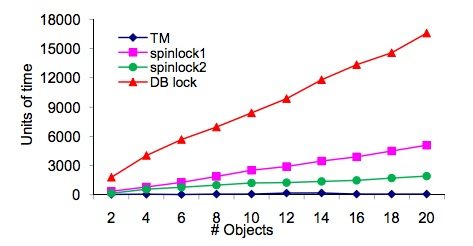
\includegraphics[width=0.45\textwidth]{figure/overhead.jpg} \caption{Overhead
%of different concurrency control protocols under low contention workloads
%\citep{tran2010}.} \label{fig:overhead} \end{figure}

%\section{Project Plan} \label{sec:plan}

Broadly speaking, we plan to:
\begin{itemize}
\item Implement two different TSX-based concurrency control protocols for
  multi-key transactions on a key-value store
\item Evaluate the performance of those schemes under different workloads
\item Compare them against pessimistic CC protocols
\end{itemize}
The goals of the project are as follows:
\begin{itemize}
\item \textbf{75\% goal:} Implement concurrency control protocol for a key-value
        store using HLE and RTM, and compare the performance of these two
        protocols.
\item \textbf{100\% goal:} Additionally, compare the above protocols with
        traditional pessimistic concurrency control protocols, specifically
        spin-locks and a lock manager. This will demonstrate the advantages of
        using HTM for this synchronization problem, or else show that 
        HTM does not help in practice.
\item \textbf{125\% goal:} Modify the HTM-based protocols to handle dynamic
        read/write sets. Alternatively, implement a software optimistic concurrency
        control protocol (like timestamp order protocol) and compare it against the
        aforementioned protocols. This would serve as a basic check that it is in
        fact the hardware, not the approach, that is the cause of any differences in
        performance.
\end{itemize}

\subsection{Resources Required}
The main resource necessary for this project is access to a machine
with a Haswell processor. We have already received access to this
resource with Dong's help.

It would be useful to have access to the existing codebase used by Prof.\ Andersen's lab to run similar HTM experiments. In particular, it would be helpful to have access to the key-value store implementation. We are expecting that Dong will be able to give us access to this, as well.

\subsection{Experiments}
Our experiments are inspired by those reported in \citep{tran2010}. We will
restrict ourselves to a small, fixed number of key-value store entries. In each
experiment, we will measure the time it takes to run a randomly generated
workload of datastore operations, given a particular concurrency control
scheme. Each workload will simply consist of looking up some set of keys and
trivially modifying their values (e.g., incrementing). Specifically, we will run
the following experiments for each type of CC mechanism:

\begin{enumerate}
\item With several fixed sizes for read/write sets and numbers of threads, vary the contention level between operations on different threads. This will allow us to determine how each of the CC mechanisms scales with respect to contention.
\item With several different fixed contention levels and numbers of threads, vary the size of the read/write sets. This will allow us to determine how each of the CC mechanisms scales with respect to the read/write set. (For HTM, this may be a very important factor, since transactions abort based on conflicts anywhere in the read/write set.)
\item With several different fixed contention levels and read/write set sizes,
    vary the number of threads running. This will allow us to determine how much benefit each mechanism is able to benefit from adding more parallelism.
\end{enumerate}

\subsection{Steps for Execution}
The required steps for executing this project are as follows:
\begin{enumerate}
\item Familiarize ourselves with an existing basic key-value store, such as that
  built by Prof.\ Andersen's group, or (if that turns out to be impractical)
  implement a simpler key-value store. In the latter case, we can
  minimize implementation effort by keeping the data structures very simple.
\item Design the structure of the transaction manager to support multiple CC mechanisms.
\item Using the Haswell TSX APIs, implement a transaction manager that optimistically attempts to execute a transaction, and retries according to either an HLE strategy or a custom RTM-specified strategy.
\item Build a system to generate test workloads with different amounts of contention. It should also allow specifying thread assignments if necessary.
\item Run the experiments for the two HTM approaches. Some tweaking will be necessary to find the most informative thread numbers, read/write set sizes, and contention levels.
\item Implement spin-locks and a lock manager.
\item Rerun the experiments for the pessimistic concurrency control approaches.
\item
  \begin{enumerate}
  \item Modify protocols for dynamic read/write sets and rerun the
    experiment using modified protocols, or
  \item Implement software-based OCC and rerun the experiments for OCC.
  \end{enumerate}
\item Collate/visualize data and write up report.
\end{enumerate}

\subsection{Progress}
As of this report's writing, we have made significant progress towards 
achieving our 100\% goal. In particular, we have implemented the following
pieces:
\begin{itemize}
\item \textbf{Key value store:} Implemented by Joy in C++, the key value store 
uses a hash table as its underlying data structure, relying on the open source
MurmurHash algorithm to hash keys. The kv store supports arbitrary keys and 
values as well as convenience methods for 64-bit integer keys and string 
values, which will be used by the testing framework. By implementing the hash 
buckets as linked lists, the kv store is safe in the face of concurrent 
insertions to the same bucket.
\item \textbf{Pessimistic locking schemes:} Implemented by Thomas, we currently 
support both spin locks and a lock table with reader/writer locks, as described 
in \Cref{sec:pessimistic}.
\item \textbf{Testing framework:} Implemented by Jesse, the testing framework 
currently acts as a sanity check to ensure that our concurrency control schemes 
are implemented correctly. It accomplishes this by spawning two threads, each 
of which repeatedly runs one transaction - a transaction that writes a random 
value to a given key, and a transaction that repeatedly reads the value of a 
single key. The reader thread then checks that the value that it read did not 
change between reads of the same transaction, ensuring that the reader and 
writer transactions were not allowed to operate on the same key concurrently.
\end{itemize}

\subsection{Completion Timeline}
Now that the fundamental pieces are in place in terms of the key value store, 
testing framework, transaction manager, and interaction between them, we have 
a few tasks left to complete before writing our final report.
\begin{itemize}
\item \textbf{HTM transaction manager:} Probably the most important remaining 
piece of the project, the HTM transaction manager will be implemented by Joy. 
We have already begun to look into the instructions necessary to make this 
work, so implementing it should be fairly straight forward, and we anticipate 
completing this by 11/16.
\item \textbf{Testing framework:} The next most important thing will be to 
flesh out the testing framework, providing support for varying the number of 
threads, level of contention in the workload, and size of the transaction's 
working sets. This will be implemented by Jesse, and should also be finished by 
11/16.
\item \textbf{Data gathering:} The final component necessary for us to reach 
our 100\% goal is to run a large number of experiments using the testing 
framework, record the data, and generate graphs as appropriate for the paper. 
A more extensive discussion of this is included in \Cref{sec:eval}. We will 
also work to refine the various CC schemes here to achieve the best performance 
possible for each. This task is assigned to Thomas, and should be completed by 
11/23.
\item \textbf{Stretch goal:} Once we have completed our 100\% goals, we will 
move on to our stretch goals. If the results of our testing indicate that HTM 
is significantly faster than the pessimistic schemes, we intend to implement 
software based OCC to determine whether the speed up is the result of the use 
of optimistic concurency control or the use of hardware based control. 
Otherwise, we will explore the effects of dynamic read/write sets on the 
performance of the different CC schemes. We will cut off work on the stretch 
goals by 12/6 to ensure we have enough remaining time to complete the final 
paper.
\item \textbf{Final Paper:} Each member of the group will be responsible for 
the sections of the paper that relate to the aspects of the project they 
implemented. We intend to finish the paper 5 minutes before the deadline.
\end{itemize}


%\section{Evaluation} \label{sec:eval}

To evaluate our algorithms, we decided to use the ``scikit-learn''
\citep{scikit-learn} package for Python. In exploring the best way to
map workloads onto benchmarks, we evaluated both clustering algorithms
as well as SVM. The rest of this section discusses the results we
observed with each method.

\begin{figure*}[h]
    \centering
    \begin{tabular}{c c c c}
      \toprule
      Algorithm                     & Homogeneity & Completeness & V-Measure \\
      \midrule
      K-Means                       & 1.000       & 1.000        & 1.000     \\
      Affinity-Propagation          & 0.824       & 1.000        & 0.904     \\
      Mean-Shift                    & 1.000       & 0.795        & 0.886     \\
      Ward Agglomerative Clustering & 1.000       & 1.000        & 1.000     \\
      DBSCAN                        & 0.000       & 1.000        & 0.000     \\
      \bottomrule
    \end{tabular}

    \caption{Clustering Algorithm Performance Metrics}
    \label{fig:clustering-metrics}
\end{figure*}

Clustering was our first approach as an unsupervised algorithm seemed
to best fit the data at hand. As such, we tried the following methods,
all of which are inbuilt in scikit-learn:

\begin{itemize}
\item K-Mean
\item Affinity Propagation
\item Mean-Shift
\item Ward Agglomerative Clustering
\item DBSCAN
\end{itemize}

The clusters found by each algorithm can be seen in
\ref{fig:clusters}. We also calculated common clustering metrics such
as homogeneity, completeness, and V-measure. These results can be
found in \ref{fig:clustering-metrics}. From the results, we notice
immediately that DBSCAN does not work well with our data. Indeed, it
does not find any distinct clusters at all. However, K-Means and Ward
Agglomerative Clustering are very good. We believe that this is
partially because both of these algorithms require number of clusters
as a parameter, which allows them to find our desired number of
clusters. However, this is not a restriction for our problem as we
know the number of benchmarks - and hence the number of clusters -
that we have.

In addition to evaluating clustering algorithms, we also evaluated
Support Vector Machines, a supervised classifier. While real-world
data will not be labeled and hence a supervised classifier cannot be
used, it is useful to see how effective our features are in
discriminating between benchmarks. Using a simple two-fold
cross-validation, we found that a simple SVM with an RBF kernel
achieved 86\% precision but with a very high standard deviation of
28\%. However, this is still a very strong result as it indicates that
our features effectively separate our data into our desired
classes. 
We plan to validate the classifier on more sophisticated heterogeneous 
real-world workloads as part of our stretch goal.

The immediate goal is to build an estimator that allows us to address the
second goal of this project. We already have the infrastructure required
for collecting metrics and features required for solving this problem.
We plan to explore different machine learning algorithms to achieve this
in the next 2 weeks.
 




\bibliographystyle{plain}
\bibliography{ref}

\end{document}
% end doc
